% =============================================================================
% Lecture 01: Introduction, Exponential Smoothing & Forecast Evaluation
% ECON 8310: Business Forecasting
% University of Nebraska at Omaha
% =============================================================================

\documentclass[aspectratio=169, 11pt]{beamer}

\input{header}

% ---- Lecture metadata --------------------------------------------------------
\title[Intro, ETS \& Evaluation]{Introduction, Exponential Smoothing \& Forecast Evaluation}
\subtitle{ECON 8310: Business Forecasting --- Lecture 1}
\author{Department of Economics}
\institute{University of Nebraska at Omaha}

% =============================================================================
\begin{document}
% =============================================================================

\begin{frame}
  \titlepage
\end{frame}

% ---- Outline ----------------------------------------------------------------
\begin{frame}{Lecture Outline}
  \tableofcontents
\end{frame}

% =============================================================================
\section{Why Forecasting Matters}
% =============================================================================

\sectionslide{Why Forecasting Matters}{%
  Every business decision made today depends on expectations about tomorrow.}

% --- Slide: The pervasiveness of forecasting ---------------------------------
\begin{frame}{Forecasting Is Everywhere in Business}
  \begin{center}
    {\small
    \begin{tabular}{p{3.3cm}p{9.6cm}}
      \toprule
      \textbf{Domain} & \textbf{The question someone is actually asking} \\
      \midrule
      Operations \& supply chain
        & How much inventory should Walmart order for Black Friday?
          How many nurses does a hospital need next Tuesday night? \\[2pt]
      Finance \& risk
        & Will credit card defaults rise next quarter?
          What will the Fed Funds rate be in six months? \\[2pt]
      Marketing \& strategy
        & How many units will this new product sell in year one?
          What is the lifetime value of this customer cohort? \\[2pt]
      Macro \& public policy
        & Will GDP grow by 2\% or 3\% next year?
          What will unemployment be in Q4? \\
      \bottomrule
    \end{tabular}
    }
  \end{center}
  \vspace{0.2cm}
  Every one of these is a \emph{decision} waiting on a number.
  \textbf{A decision is only as good as the forecast it rests on.}
\end{frame}

% --- Slide: Forecasting setup ------------------------------------------------
\begin{frame}{The Basic Setup}
  \begin{definitionbox}{Time Series}
    A \key{time series} is an ordered sequence of observations
    $\{y_1, y_2, \ldots, y_T\}$ where $t$ indexes time.
  \end{definitionbox}
  \textbf{Notation for the whole course:}
  \begin{itemize}\small\itemsep1pt
    \item $y_t$ --- observed value at time $t$
    \item $h$ --- \key{forecast horizon}: harder as $h$ grows, as uncertainty compounds
    \item $\hat{y}_{t+h|t}$ --- forecast of $y_{t+h}$ made using information at time $t$
    \item $e_t = y_t - \hat{y}_{t|t-1}$ --- \key{forecast error}
  \end{itemize}
  \vspace{0.15cm}
  Under squared-error loss the best forecast is the \textbf{conditional
  expectation}, $\hat{y}_{t+h|t} = \mathbb{E}[y_{t+h} \mid \mathcal{F}_t]$,
  where $\mathcal{F}_t$ is everything known at time $t$.
\end{frame}

% --- Slide: Time series components -------------------------------------------
\begin{frame}{Components of a Time Series}
  Any series can be decomposed into four parts (additive form):
  $y_t = T_t + S_t + C_t + I_t$.
  \begin{itemize}\small\itemsep1pt
    \item \key{$T_t$ Trend} --- long-run direction
    \item \key{$S_t$ Seasonality} --- regular, calendar-driven pattern
    \item \key{$C_t$ Cycle} --- medium-run business-cycle swings
    \item \key{$I_t$ Irregular} --- random shocks
  \end{itemize}
  Which parts matter depends on the series: retail sales are trend $+$
  seasonality, quarterly GDP is trend $+$ cycle, daily stock returns are
  mostly irregular.
  \begin{warningbox}
    \textbf{Ignoring seasonality causes large, systematic errors.}
    A non-seasonal model on monthly retail data will consistently
    under-forecast December and over-forecast January --- every single year.
  \end{warningbox}
\end{frame}

% --- Slide: Naive benchmarks -------------------------------------------------
\begin{frame}{Always Beat a Benchmark First}
  Before presenting any forecast model, check that it beats a \textbf{naive
  benchmark}. A model that cannot beat the baseline has zero value.
  \begin{center}
    {\small
    \begin{tabular}{llp{6.2cm}}
      \toprule
      \textbf{Benchmark} & \textbf{Forecast} & \textbf{Use when} \\
      \midrule
      Na\"{i}ve          & $\hat{y}_{t+h|t} = y_t$            & Asset prices, random walks \\
      Seasonal na\"{i}ve & $\hat{y}_{t+h|t} = y_{t+h-m}$      & Any series with a season \\
      Mean               & $\hat{y}_{t+h|t} = \bar{y}_t$      & No trend, no season \\
      Drift              & $\hat{y}_{t+h|t} = y_t + h\hat{c}$ & Trend, no season \\
      \bottomrule
    \end{tabular}
    }
  \end{center}
  \vspace{0.1cm}
  \muted{\small This is not a formality. In the M4 Competition many machine
  learning models \emph{failed} to beat simple exponential smoothing
  \parencite{Makridakis2020}.}
\end{frame}

% =============================================================================
\section{Exponential Smoothing}
% =============================================================================

\sectionslide{Exponential Smoothing}{%
  Recent observations should carry more weight than old ones.}

% --- Slide: The equal-weight problem -----------------------------------------
\begin{frame}{The Problem with Equal Weights}
  Most classical methods weight every observation equally --- but what if the
  world \textbf{changes}? After a store renovation, equal weights keep
  forecasting the old store for months.

  \vspace{0.1cm}
  \textbf{Exponential weighting:} an observation $k$ weeks old gets weight
  $\alpha(1-\alpha)^k$. High $\alpha$ = short memory; low $\alpha$ = long memory:
  \begin{center}
    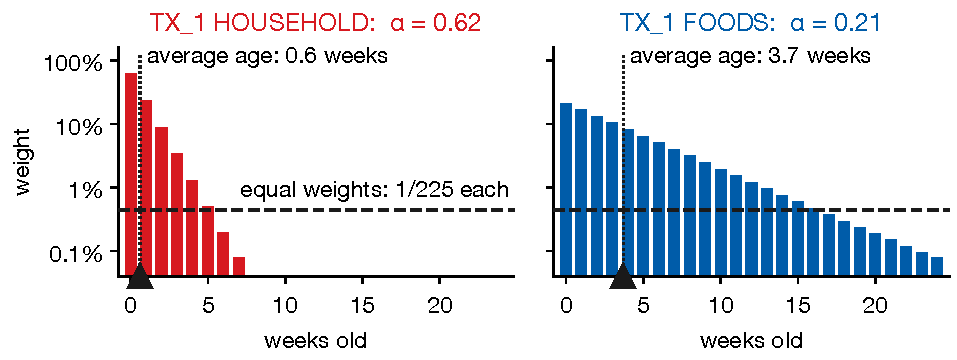
\includegraphics[height=3.65cm]{../Figures/Lecture01_ETS_Eval/ses_weights.pdf}
  \end{center}
  \vspace{-0.35cm}
  \muted{\small Fitted $\alpha$ on two aisles of one store. Log scale: each week
  back is the same step down, $\times(1-\alpha)$.}
\end{frame}

% --- Slide: SES ---------------------------------------------------------------
\begin{frame}{Simple Exponential Smoothing (SES)}
  \begin{definitionbox}{SES Update Equation}
    The \textbf{level} $\ell_t$ closes the fraction $\alpha$ of each week's gap
    ($0 < \alpha \leq 1$); the forecast is flat.\par\vspace{3pt}
    \centerline{$\ell_t = \alpha\, y_t + (1-\alpha)\,\ell_{t-1}
             = \ell_{t-1} + \alpha\,(y_t - \ell_{t-1}),
      \qquad \hat{y}_{T+h|T} = \ell_T$}
  \end{definitionbox}
  \vspace{-0.15cm}
  \begin{center}
    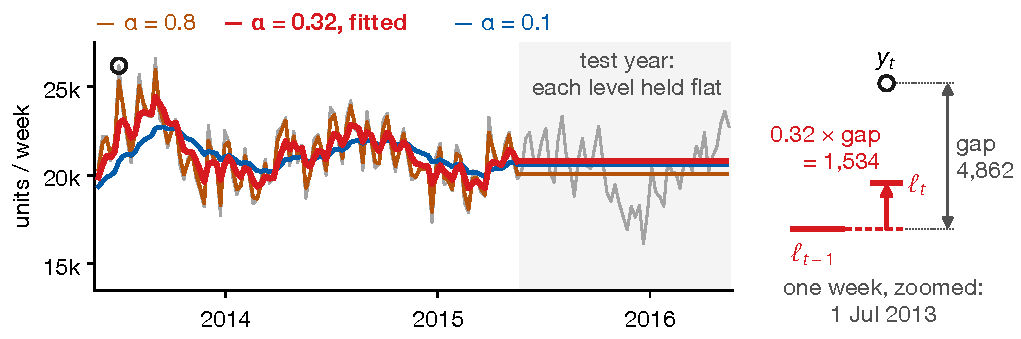
\includegraphics[height=3.45cm]{../Figures/Lecture01_ETS_Eval/ses_levels.pdf}
  \end{center}
  \vspace{-0.35cm}
  {\small Large $\alpha$ chases every wiggle; small $\alpha$ is smooth but slow.
  SES \textbf{nests both benchmarks}: $\alpha = 1$ is na\"{i}ve, $\alpha \to 0$ the
  historical mean.} \muted{\footnotesize\itshape No trend, no season.}
\end{frame}

% --- Slide: Holt ---------------------------------------------------------------
\begin{frame}{Holt's Method: Adding Trend}
  SES is \emph{flat}. For a trending series, track the level $\ell_t$ and the slope $b_t$:
  \begin{definitionbox}{Holt's Linear Exponential Smoothing \parencite{Holt2004}}
    {\small
    \textbf{Level:} $\;\ell_t = \alpha\, y_t + (1-\alpha)\,(\ell_{t-1} + b_{t-1})$\\[2pt]
    \textbf{Trend:} $\;b_t = \beta^*(\ell_t - \ell_{t-1}) + (1-\beta^*)\,b_{t-1}$\\[2pt]
    \textbf{Forecast:} $\hat{y}_{T+h|T} = \ell_T + h\,b_T$
    }
  \end{definitionbox}
  \begin{columns}[c]
    \begin{column}{0.40\textwidth}
      \textbf{Straight lines get unrealistic far out.} For $h > 6$, the
      \textbf{damped trend} multiplies each week's rise by $\phi$ ($0 < \phi < 1$),
      so the forecast levels off under $\ell_T + b_T\,\phi/(1-\phi)$.
    \end{column}
    \begin{column}{0.58\textwidth}
      \centering
      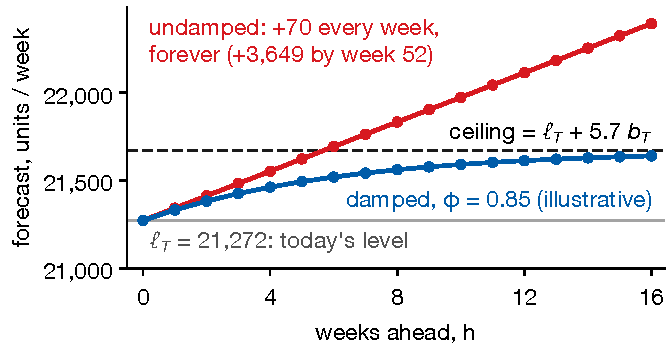
\includegraphics[height=3.6cm]{../Figures/Lecture01_ETS_Eval/damped_trend.pdf}
    \end{column}
  \end{columns}
\end{frame}

% --- Slide: Holt-Winters -------------------------------------------------------
\begin{frame}{Holt-Winters: Level, Trend, and Seasonality}
  \begin{definitionbox}{Holt-Winters Additive Method \parencite{Winters1960}}
    {\small
    \vspace{-0.1cm}
    \[
    \begin{aligned}
      \ell_t &= \alpha(y_t - s_{t-m}) + (1-\alpha)(\ell_{t-1}+b_{t-1}) \\[-1pt]
      b_t &= \beta^*(\ell_t - \ell_{t-1}) + (1-\beta^*)\,b_{t-1} \\[-1pt]
      s_t &= \gamma(y_t - \ell_{t-1} - b_{t-1}) + (1-\gamma)\,s_{t-m} \\[-1pt]
      \hat{y}_{T+h|T} &= \ell_T + h\,b_T + s_{T+h-m}
      \qquad (m = \text{seasonal period})
    \end{aligned}
    \]
    \vspace{-0.4cm}
    }
  \end{definitionbox}
  \begin{columns}[T]
    \begin{column}{0.48\textwidth}
      \textbf{Additive seasonality:}
      \begin{itemize}\small\itemsep0pt
        \item Swings constant in size: the same $\pm$ amount every December
      \end{itemize}
    \end{column}
    \begin{column}{0.48\textwidth}
      \textbf{Multiplicative seasonality:}
      \begin{itemize}\small\itemsep0pt
        \item Swings grow with the level: retail sales, tourism
      \end{itemize}
    \end{column}
  \end{columns}
  \vspace{0.2cm}
  US retail's December spike grows as overall sales grow: \textbf{multiplicative}.

  \muted{\footnotesize Needs at least $2m$ observations to initialize
  ($m=12$ for monthly data).}
\end{frame}

% --- Slide: ETS framework -----------------------------------------------------
\begin{frame}{The ETS Framework: A Unified View}
  \textcite{Hyndman2021} unify every exponential smoothing method as a
  \textbf{state space model}: Error $\times$ Trend $\times$ Seasonal.
  \begin{center}
    {\small
    \begin{tabular}{lll}
      \toprule
      \textbf{Component} & \textbf{Options} & \textbf{Meaning} \\
      \midrule
      Error ($E$)    & A, M & Additive / Multiplicative \\
      Trend ($T$)    & N, A, A\textsubscript{d} & None / Additive / Damped \\
      Seasonal ($S$) & N, A, M & None / Additive / Multiplicative \\
      \bottomrule
    \end{tabular}
    }
  \end{center}
  That is 18 combinations; three are numerically unstable, which leaves 15.
  Ours are among them: \textbf{ETS(A,N,N)} is SES, \textbf{ETS(A,A,N)} is Holt
  linear, \textbf{ETS(A,A\textsubscript{d},N)} is Holt damped,
  \textbf{ETS(A,A,A)} is Holt-Winters additive, and \textbf{ETS(M,A,M)} is
  Holt-Winters multiplicative.

  \vspace{0.15cm}
  \textbf{Automatic selection:} fit all 15 and pick the minimum AIC. In Python,
  \texttt{statsmodels.tsa.exponential\_smoothing.ets.ETSModel}.
\end{frame}

% =============================================================================
\section{Forecast Evaluation}
% =============================================================================

\sectionslide{Forecast Evaluation}{%
  Forecasting without evaluation is not science --- it is storytelling.}

% --- Slide: Accuracy metrics ---------------------------------------------------
\begin{frame}{How Do We Measure Forecast Accuracy?}
  Draw each out-of-sample error $e_{T+h} = y_{T+h} - \hat{y}_{T+h|T}$ as a
  square. CA\_1 FOODS, the 52 test weeks:
  \begin{columns}[c]
    \begin{column}{0.36\textwidth}
      \[
        \MAE  = \tfrac{1}{H}\textstyle\sum_{h=1}^{H} |e_{T+h}|
      \]
      \vspace{-0.5cm}
      \[
        \RMSE = \sqrt{\tfrac{1}{H}\textstyle\sum_{h=1}^{H} e_{T+h}^2}
      \]
      {\small MAE is the average \textbf{side} (dashed). RMSE is the side of the
      average \textbf{square} (filled), so $\RMSE \geq \MAE$.}
    \end{column}
    \begin{column}{0.62\textwidth}
      \centering
      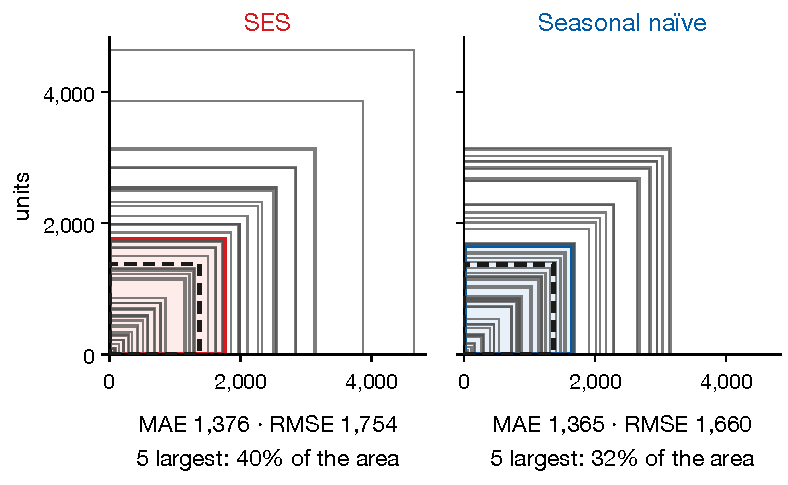
\includegraphics[height=5.0cm]{../Figures/Lecture01_ETS_Eval/error_squares.pdf}
    \end{column}
  \end{columns}
  \vspace{0.1cm}
  {\small A tie on MAE, not on RMSE: five big misses carry 40\% of SES's squared
  error. When big misses are costly --- a stockout --- prefer RMSE.}
\end{frame}

% --- Slide: Scale-free metrics --------------------------------------------------
\begin{frame}{Comparing Across Series: MAPE and MASE}
  RMSE and MAE come in the units of $y_t$, so they compare models on the
  \emph{same} series. To compare \emph{across} series, scale the errors:
  \[
    \text{MAPE} = \frac{100\%}{H}\sum_{h=1}^{H}
                  \left|\frac{e_{T+h}}{y_{T+h}}\right|
    \qquad\qquad
    \text{MASE} = \frac{\MAE}{\displaystyle\frac{1}{T-m}\sum_{t=m+1}^{T} |y_t - y_{t-m}|}
  \]
  The MASE denominator is seasonal na\"{i}ve's average miss \textbf{on the
  training data}. $\text{MASE} < 1$: smaller errors than that;
  $\text{MASE} > 1$: \negc{worse}. It is the standard in the M-Competitions
  \parencite{Makridakis2020}.

  \vspace{0.15cm}
  \muted{\small MAPE breaks down when $y_t$ is near zero; MASE does not.}
\end{frame}

% --- Slide: Out-of-sample principle -------------------------------------------
\begin{frame}{The Golden Rule: Always Evaluate Out-of-Sample}
  \textbf{Never evaluate a forecast model on the data used to fit it.}
  In-sample fit measures how well the model memorized the past, not how well
  it predicts the future.
  \begin{center}
    \begin{tikzpicture}[scale=0.9]
      \draw[->, thick, color=unoblack] (0,0) -- (11,0) node[right] {$t$};
      \fill[unolightgray] (0.1, 0.2) rectangle (7.5, 0.8);
      \draw[unoblack, thick] (0.1, 0.2) rectangle (7.5, 0.8);
      \node at (3.8, 0.5) {\textbf{Training set}};
      \node[below, color=unogray, font=\small] at (0.1, -0.1) {$t=1$};
      \node[below, color=unogray, font=\small] at (7.5, -0.1) {$t=T$};
      \fill[unolightred] (7.5, 0.2) rectangle (10.5, 0.8);
      \draw[unored, thick] (7.5, 0.2) rectangle (10.5, 0.8);
      \node at (9.0, 0.5) {\textbf{Test set}};
      \node[below, color=unogray, font=\small] at (10.5, -0.1) {$t=T+H$};
      \draw[dashed, color=unored, thick] (7.5, -0.05) -- (7.5, 1.2);
      \node[above, color=unored] at (7.5, 1.2) {\footnotesize Forecast origin};
    \end{tikzpicture}
  \end{center}
  \begin{warningbox}
    \textbf{Never randomly shuffle time series observations.} Use
    \texttt{TimeSeriesSplit} in scikit-learn, never \texttt{KFold}. Shuffling
    lets future data train the model --- data leakage that makes results look
    excellent and forecast badly.
  \end{warningbox}
\end{frame}

% =============================================================================
\section{Course Roadmap}
% =============================================================================

\sectionslide{Course Roadmap}{%
  What we will cover, and how it fits together.}

% --- Slide: Course structure -------------------------------------------------
\begin{frame}{ECON 8310: Four-Part Structure}
  \begin{center}
    {\small
    \begin{tabular}{p{3.1cm}p{9.8cm}}
      \toprule
      \textbf{Part} & \textbf{Lectures} \\
      \midrule
      I. Time series
        & 1. Intro, ETS \& evaluation \muted{$\leftarrow$ today} \quad
          2. ARIMA \& VAR \quad
          3. Generalized additive models \\[2pt]
      II. Tree-based
        & 4. Decision trees \quad
          5. Tree ensembles: random forests \& boosted trees \quad
          6. Regularization \& model selection \\[2pt]
      III. Deep learning
        & 7. Neural networks (PyTorch) \quad
          8. CNN architectures \quad
          9. RNNs, LSTMs \& Transformers \\[2pt]
      IV. Bayesian
        & 10. Foundations \quad
          11. Time series \& hierarchical models \quad
          12. Bayesian linear regression \\
      \bottomrule
    \end{tabular}
    }
  \end{center}
  \vspace{0.1cm}
  \muted{\small Python throughout: statsmodels, scikit-learn, xgboost, PyTorch,
  prophet, pyGAM, pymc.}
\end{frame}

% --- Slide: Tools and expectations -------------------------------------------
\begin{frame}{Tools and What You Will Be Able to Do}
  \textbf{The Python stack:} \texttt{statsmodels} (ETS, ARIMA, VAR) $\cdot$
  \texttt{scikit-learn} (models, pipelines, cross-validation) $\cdot$
  \texttt{xgboost} (gradient boosting) $\cdot$ \texttt{torch} (neural networks)
  $\cdot$ \texttt{prophet} and \texttt{pygam} (GAMs) $\cdot$ \texttt{pymc}
  (Bayesian models).

  \vspace{0.25cm}
  \textbf{By the end of the semester you will be able to:}
  \begin{itemize}\itemsep2pt
    \item[\pos{$\checkmark$}] Choose the right method for a given business problem
    \item[\pos{$\checkmark$}] Implement and tune it in Python
    \item[\pos{$\checkmark$}] Evaluate it rigorously out-of-sample
    \item[\pos{$\checkmark$}] Interpret the result for a non-technical stakeholder
    \item[\pos{$\checkmark$}] Use AI tools effectively to accelerate the analysis
    \item[\pos{$\checkmark$}] Avoid the most common forecasting mistakes
  \end{itemize}
\end{frame}

% --- Slide: Key Takeaways -----------------------------------------------
\begin{frame}{Lecture 1: Key Takeaways}
  \begin{keybox}
    {\small
    \begin{enumerate}
      \item Under squared loss the best forecast is the
            \textbf{conditional expectation}.

      \item \textbf{Always beat a benchmark first:}
            na\"{i}ve, seasonal na\"{i}ve, mean, drift.

      \item Exponential smoothing weights the past \textbf{geometrically};
            $\alpha$ sets how fast it forgets.

      \item SES $\to$ Holt (+ trend) $\to$ Holt-Winters (+ season): all
            \textbf{ETS} models, chosen by AIC.

      \item \textbf{Evaluate out-of-sample, never shuffled.} RMSE punishes big
            misses; MASE compares across series.
    \end{enumerate}
    }
  \end{keybox}
  \muted{\itshape Next: ARIMA \& VAR ---
  a regression-based approach to time series with rich autocorrelation structure.}
\end{frame}

% --- References ---------------------------------------------------------------
\begin{frame}[allowframebreaks]{References}
  \printbibliography[heading=none]
\end{frame}

% =============================================================================
\end{document}
% =============================================================================
